\dev{Emile Martinez}{}{}{}

\section{Dictionnaire : type abstraits et motivation}


\begin{definition}[Dictionnaire]
	Soit $X$ un ensemble d’éléments appelés valeurs, et $K$ un ensemble d’éléments appelés clés. Un dictionnaire $D$ est une structure de données abstraites ayant les trois opérations :
	
	— $\texttt{Inserer}(D,k,x)$ : insère le couple $(k, x)$ dans $D$, en écrasant un éventuel couple $(k, x')$ préexistant.
	
	— $\texttt{Recherche}(D,k)$ : renvoie la valeur de $x$ telle que $(k, x)$ est dans $D$, si elle existe (peut renvoyer une valeur pas dans $X$ sinon)
	
	— $\texttt{Supprime}(D,k)$ supprime un éventuel couple $(k, x)$ présent dans $D$.
\end{definition} 

\begin{example}
	annuaire téléphonique : les clefs sont les noms des personnes, les valeurs leurs numéros de téléphone
\end{example}

\begin{rem}
	Les dictionnaires sont aussi appelés tableaux associatifs
\end{rem}

\begin{appl}
	Si on a une base de données de personnes, identifiés par un pseudonyme, on peut stocker leur informations dans un dictionnaire.
\end{appl}

\begin{rem}
	C'est ce qui se passe dans une base de données
\end{rem}

\begin{impl}[naive]
	On pourrait stocker tous les éléments dans une liste, sans ordre particulier
\end{impl}

\begin{exercise}
	Implémenter alors les fonctions de bases. Quelles sont leur complexité ?
\end{exercise}

\section{Implémentation}

\subsection{Par des arbres}

\subsubsection{Arbres binaires de recherche (ABR)}

\begin{definition}[ABR]
	Un arbre binaire de recherche (ABR) est un arbre binaire dont les éléments sont munis d'un ordre total et où, pour chaque sous-arbre $N(g, x, d)$, l'élément $x$ est supérieur à tous les éléments de $g$ et inférieur à tous les éléments de $d$.
\end{definition}

\begin{impl}
	On peut implémenter un dictionnaire à l'aide d'un ABR à condition que l'ensemble des clefs soit muni d'un ordre total (On insère les couples (clé, valeur) et l'ordre est sur les valeurs)
\end{impl}

\begin{example} Deux implémentations du même ABR :\\
	\begin{minipage}{0.5\linewidth}
		\begin{tikzpicture}[-, node distance=2cm]
			\node[state] (q0) {10};
			\node[state, below left of = q0] (q1) {8};
			\node[state, below left of = q1] (q2) {5};
			\node[state, below left of = q2] (q3) {3};
			
			\draw (q0) edge[] node{} (q1);
			\draw (q1) edge[] node{} (q2);
			\draw (q2) edge[] node{} (q3);
			
		\end{tikzpicture}
	\end{minipage}\begin{minipage}{0.5\linewidth}
		\begin{tikzpicture}[-, node distance=2cm]
			\node[state] (q0) {5};
			\node[state, below left of = q0] (q1) {3};
			\node[state, below right of = q0] (q2) {10};
			\node[state, below left of = q2] (q3) {8};
			
			\draw (q0) edge[] node{} (q1);
			\draw (q0) edge[] node{} (q2);
			\draw (q2) edge[] node{} (q3);
			
		\end{tikzpicture}
	\end{minipage}
\end{example}

\paragraph{Insertion} Dans un ABR, on insère un élément $x$ en descendant depuis la racine, en prenant le fils gauche ou le fils droit selon si $x$ est plus petit ou plus grand que la racine courante, et en créant un nouveau nœud étiqueté par $x$ lorsque l’on ne peut plus avancer.
	
\paragraph{Recherche} Elle se fait de manière analogue

\paragraph{Suppression} Lorsque le nœud est une feuille ou si le nœud n’a qu’un enfant, alors la transformation est simple. Par contre, si le nœud possède deux enfants, alors il faut retirer le minimum du sous-arbre droit (ou le maximum du sous-arbre gauche) pour le remplacer.

\begin{exercise}
	Implémentation des ABR en OCamL
\end{exercise}

\begin{proposition}
	Soit $\mathcal A$ un ABR à $n$ nœuds et de hauteur $h$. La recherche, l’insertion et la suppression	se font dans le pire cas en $O(h)$ comparaisons. Or un ABR peut être déséquilibré : la hauteur est alors en $O(n)$
\end{proposition}

\subsubsection{Arbres rouge-noir (ARN)}

\begin{definition}
	 Un arbre rouge noir (ARN) est un ABR où chaque nœud porte une couleur rouge ou noir, et qui vérifie les deux propriétés suivantes : \begin{itemize}
		\item la racine est noire 
		\item les potentiels fils d'un nœud rouge sont noirs
		\item pour chaque nœud, tous les chemins menant de ce nœud à une feuille ont le même nombre de nœuds noirs. 
	\end{itemize}
\end{definition}

\begin{proposition}
	\label{06-equilibre}
	Les ARN sont équilibrés ($h = O(\log n)$)
\end{proposition}

\begin{corollary}
	Dans un ARN, on peut effectuer les opérations d'insertion, de recherche et de suppression en $O(h)$, ie $O(\log n)$. 
\end{corollary}

\paragraph{Developpement} Preuve de la propriété \ref{06-equilibre} et présentation de l'insertion dans un ARN

\subsection{Tables de hachage}

\begin{idee}
	Le but ici va être de stocker nos données dans un tableau (d'où le nom tableau associatif). Cela se fait donc en deux étapes : \begin{itemize}
		\item Associer à notre données un nombre (pas trop grand) (appelé hachage) par une fonction appelée fonction de hachage.
		\item Avoir un tableau avec une case par hachage possible, où l'on stocke la donnée
	\end{itemize}
\end{idee}

\subsubsection{Fonction de hachage}

\begin{definition}
	Une fonction de hachage est une fonction $h : K \to \llbracket 0, m-1 \rrbracket$ (avec $m << |K|$)
\end{definition}

\begin{proposition}
	Une fonction de hachage a la propriété du hachage parfait si pour $x \neq y \in K$, $\mathbb P(h(x) = h(y)) = \dfrac{1}{m}$
\end{proposition}

\begin{rem}
	Le hachage parfait veut dire que les valeurs de hachage sont comme pris au hasard dans $\llbracket 0, m-1\rrbracket$. Néanmoins, comme on veut que $h(x)$ vaille toujours la même chose, on ne prend pas de fonctions aléatoires.
\end{rem}

\begin{example}
	On choisit un flottant A. On interprète les bits de données de la structure comme un entier x (en les collant). On prend alors $h(d) = \lfloor A*x \rfloor \mod m$
\end{example}

\subsubsection{Table de hachage}

Il y a trois étapes dans le stockage dans un tableau: \begin{enumerate}
	\item Hacher la valeur et la mettre dans à sa case dans le tableau
	\item Si la case était déjà occupée (collision), stocker la donnée dans une structure annexe
	\item Si le tableau est trop plein, augmenter m (et donc recopier toutes les données).
\end{enumerate}

\begin{example} Schéma où la structure annexe est une liste chaînée pour chaque case\\
	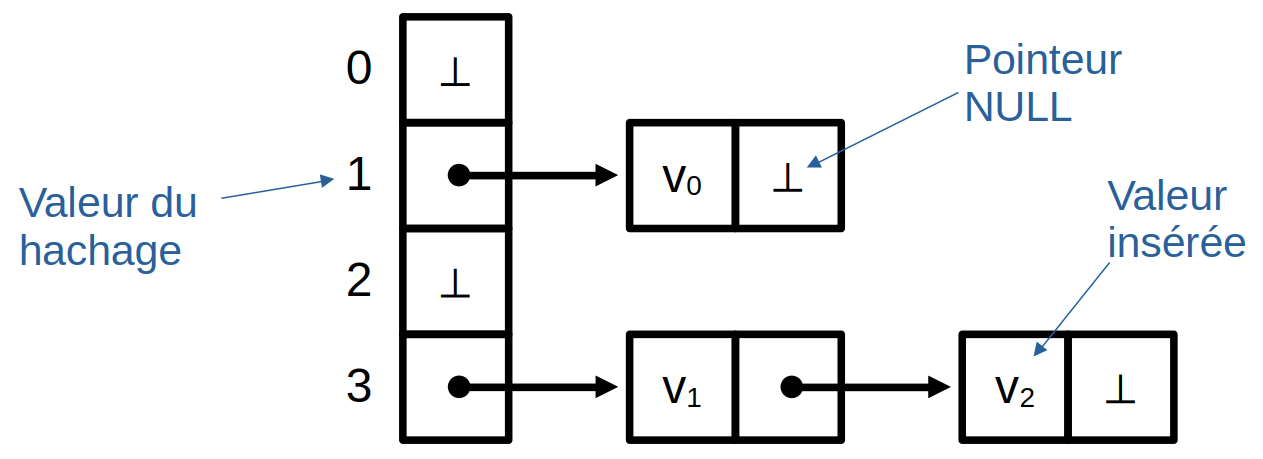
\includegraphics[width = 0.7\linewidth]{lecon/06-ensembles_et_dictionnaires/table_hachage.png}
\end{example}

\begin{com}
	Si on a la place on peut ecrire la remarque, sinon le dire à l'oral que si les abr nécessite un ordre total, la table de hachage nécessite de sérialiser ou de donner directement le hachage
\end{com}

\begin{com}
	Normalement là on pourrait parler de compexité, mais on considère que le tableau \ref{06-tab} suffit.
\end{com}

\section{Ensembles}

\begin{definition}
	Un ensemble est un dictionnaire dans lequel il n'y a pas de clefs. La fonction recherche renvoie donc un booléen qui indique la présence ou non de l'élément. 
\end{definition}

\begin{rem}
	On déduit alors de l'implémentation des dictionnaires, l'implémentation des ensembles
\end{rem}

\begin{com}
	Cette remarque justifie que l'on parle si brièvement des ensembles, et si tard dans la leçon. Beaucoup des choses sur les ensembles se déduisant de celles des dictionnaires
\end{com}

\begin{idee}
	Comme ce sont des ensembles on pourrait également vouloir des opérations ensemblistes comme l'union, l'intersection, etc...
\end{idee}

\begin{impl}
	On peut faire ces opérations sur les structures précédentes en les parcourant (pour l'union, on insère tous les éléments de l'un dans l'autre par exemple)
\end{impl}

\begin{rem}
	Ces opérations réhabilite l'idée de la liste triée
\end{rem}

Récapitulatif des complexités :\\


\begin{tabular}{|l|c|c|c|c|c|}
	\hline \label{06-tab} Structure & Insertion & Suppression & Recherche & union & intersection\\
	\hline liste & $O(n)$ & $O(n)$ & $O(n)$ & $O(n\times m)$ & $O(n \times m)$ \\
	\hline liste triée & $O(n)$ & $O(n)$ & $\log n$ & $O(n+m)$ & $O(n+m)$\\
	\hline ARN & $O(\log n)$ & $O(\log n)$ & $O(\log n)$ & $O(n+m)\log(n+m)$ & $O(\min(n,m) \log(\max(n,m)))$\\
	\hline Table de  & $O(n)$ & $O(n)$ & $O(n)$ & $O(n\times m)$ & $O(n \times m)$ \\
	hachage & $O(1)$ moy. & $O(1)$ moy. & $O(1)$ moy. & $O(n+m)$ moy. & $O(\min(n,m))$ moy. \\ \hline 
\end{tabular}

\begin{exercise}
	Choisir des implémentations en C et les comparer. Si l'on traite les listes triées, ouverture sur les skip listes
\end{exercise}

\section{Application}

\subsection{Dictionnaire d'adjacence}

Soit $G=(S, A)$ un graphe. (où $S = \llbracket 1, n \rrbracket$)\\

On peut représenter $G$ par un tableau de dictionnaire $D$ tq $D[u]$ est un dictionnaire contenant les voisins de $u$\\

\textbf{intérêts :} On a les avantages de la matrice d'adjacence (on detecte rapidement si il y a une arête) et des listes d'adjacence (stockage en |A| et obtention de tous les voisins linéairement).\\

\begin{example}
	Sur un graphe de personnes se connaissant, on sait si A connait B rapidement, mais on n'a pas à stocker tous les false des couples de personnes en se connaissant pas.
\end{example}

\subsection{Mémoïsation}
Supposons que l'on ait une fonction du type
\begin{lstlisting}
fonction (f_args):
    corps de f
    return x
\end{lstlisting}

Il se peut que l'on ait beaucoup d'appels à \texttt f sur les mêmes arguments, comme des fonctions récurisves en programmation dynamique. En s'inspirant de cette dernière, on peut alors ne faire qu'une fois les appels sur chaque argument grâce à un dictionnaire :

\begin{lstlisting}
fonction f(args):
    Si args est dans dictionnaire:
        renvoyer dictionnaire[args]
    Sinon:
        corps de f
    dictionnaire[args] = x
    renvoyer x
\end{lstlisting}

\subsection{Autres applications}

\begin{com}
	On peut dire à l'oral que en gros, utiliser un dictionnaire est un peu équivalent à $f : K \to \llbracket 1, K \rrbracket$. (c'est plus que simplement le fait logique que, par un tableau classique, c'est équivalent)
\end{com}

Les dictionnaires et les ensembles servent dès que l'on veut accéder rapidement à un élément dont la structure n'est pas un entier.

\begin{example}
	En algorithmique du texte, pour associer des valeurs à des chaînes de caractère (Huffman, Boyer-Moore)
\end{example}

\begin{example}
	Quand on fait un parcours de graphe dont les sommets ne sont pas $\llbracket 1, n \rrbracket$ on peut utiliser un ensemble pour savoir quels éléments on a déjà parcouru.
\end{example}

\begin{com}
	On peut soit insister à l'oral sur cet exemple, soit en faire une sous partie, du fait que c'est une application pour les ensembles
\end{com}

Mais on peut les retrouver également dans beaucoup de domaines comme en bases de données, et dès que l'on manipule un nombre faible de valeur comparés à l'ensemble des valeurs possibles.

\textbf{Développement :} Amélioration du tri par comptage par l'usage de dictionnaires.